\documentclass[usenatbib]{mnras}
\usepackage[T1]{fontenc}
\usepackage{ae,aecompl}

\usepackage{graphicx}	% Including figure files
\usepackage{amsmath}	% Advanced maths commands
\usepackage{amssymb}	% Extra maths symbols
\usepackage{array}

\usepackage{multirow}
\usepackage{multicol}
\usepackage{blindtext}
\newcolumntype{?}{!{\vrule width 1pt}}

\newcommand{\hMpc}{{\ifmmode{\ h^{-1}{\rm Mpc}}\else{$h^{-1}$Mpc\ }\fi}}  
\newcommand{\hGpc}{{\ifmmode{\ h^{-1}{\rm Gpc}}\else{$h^{-1}$Gpc\ }\fi}}  
\newcommand{\hmpc}{{\ifmmode{\ h^{-1}{\rm Mpc}}\else{$h^{-1}$Mpc\ }\fi}}  
\newcommand{\hkpc}{{\ifmmode{\ h^{-1}{\rm kpc}}\else{$h^{-1}$kpc\ }\fi}}  
\newcommand{\hMsun}{{\ifmmode{\ h^{-1}{\rm {M_{\odot}}}}\else{$h^{-1}{\rm{M_{\odot}}}$}\fi}}  
\newcommand{\kms}{{\ifmmode{\ {\rm km\, {s}^{-1}}}\else{\ km s$^{-1}$}\fi}}  

%%%%%%%%%%%%%%%%%%% TITLE PAGE %%%%%%%%%%%%%%%%%%%
\title[Our peculiar motion across the Universe]{Our peculiar motion across the Universe}
\author[Pe\~naranda-Rivera et al.]{
\parbox[t]{\textwidth}{
    {J. E. Forero-Romero $^{1}$}
    {D. Sierra$^{1}$,}
}
\\\\
$^{1}$ Departamento de F\'isica, Universidad de los Andes, Cra. 1
  No. 18A-10 Edificio Ip, CP 111711, Bogot\'a, Colombia \\
}

% These dates will be filled out by the publisher
\date{Accepted XXX. Received YYY; in original form ZZZ}

% Enter the current year, for the copyright statements etc.
\pubyear{2019}


% Don't change these lines
\begin{document}
\label{firstpage}
\pagerange{\pageref{firstpage}--\pageref{lastpage}}
\maketitle

%%%%%====MYMARK========
\maketitle
\begin{abstract}
The kinematic for binary halo samples in Local Group (LG) is not significantly different from the dynamic properties of high-precision simulations from mock catalogs. Objects in LG show a peculiar relative radial velocity distribution (related to mass of the distributions) that does not differ from simulated generic samples. From halos simulations from the Abacus project catalogs and use a standards ``Friend-of-Friend'' algorithms, we determined kinematic properties of the halos that can correspond to the main objects of the LG. For these models, we measure velocity dispersions for individual and paired halos between $242.24-649.28)$ \kms and $236.18-607.56$ \kms, respectively, many times greater than the observed values. Despite the fact that CMB models and high precision simulations may fail to produce environments similar to those of the local group on scales of a little Mpc, they undoubtedly can account for orbital properties similar to those found in pairs of type MW and M31.   
\end{abstract}

\begin{keywords}
%%PREGUNTAR
%galaxies:supercluster --- simulation:cosmological --- filter:gaussian --- methods:numerical
\end{keywords}


%=========================================================================
%		PAPER CONTENT
%=========================================================================

%*************************************************************************
\section{Introduction}
The recent discovery of the Cosmic Microwave Background (CMB) has provided sufficient evidence to accept that on megaparsec scales the matter distribution of the Universe is not
uniform and exhibits a peculiar movement in terms of relative speeds of several hundred \kms, taking into account orbital velocities of the sun in our milky way and the interaction itself with the Andromeda galaxy. For the measurement of peculiar velocities it is required that precisely distances to the galaxies can be determined. In the case of relative distances the task is simple, however measuring absolute distances is still a problem.

N-body simulations have shown that a large part of the total volume fraction of the universe is confined to hollow regions while about half of the total mass is confined to other regions called filaments \cite{2014MNRAS.441.2923C}. These simulations can determine the relative speeds between filaments and their walls confirming values close to those deduced from CMB.

\textcolor{red}{Large Peculiar Velocities have been measured in the Hydra-Centaurus Supercluster \cite{1989ApJ...338..654A} (Parkes radio telescope $\sim$ 500 \kms), in the Leo Spur \cite{2015ApJ...805..144K} (Hubble Space Telescope Advance Camera for Surveys $\sim$ 259 \kms), in the Perseus-Pisces Supercluster \cite{1992ApJ...396..453H} (Photometric measure $\sim$ 400 \kms), and beyond of local void \cite{2008ApJ...676..184T} (Nearby Galaxies Catalog \cite{1988ngc..book.....T} $\sim$ 631 \kms), are only some examples.}

Our analysis involves the application of the N-body simulation data products from the Abacus project, including halos catalogs, to high resolution and large volume cosmological simulations. The advantages offered by the N-body simulations is the possibility of including different cosmologies by varying the parameters of the cosmological model in terms of $H_0$, $w_0$, $\Omega_{CDM}h^2$, $\omega_bh^2$, $\sigma_8$, and $n_s$. many possibilities can be studied for ranges: $61.56746<H_0<74.79261$, $-1.37035<w_0<-0.6548324$, $0.1044778<\Omega_{CDM}h^2<0.132191$, $0.02085082<\omega_bh^2<0.02349378$, $0.6466325<\sigma_8<0.9986873$, and $0.9300325<n_s<0.9897832$, respectively.


\section{Numerical Setup}

We use simulations boxes from the Abacus project \cite{abacus}.  Each box has a size of $L_{\rm box}=720$ \hMpc and was simulated with $1440^3$ particles and a resulting particle mass of $\sim 1\times 10^{10}$ \hMpc. Each box also have 41 different $\omega_{CDM}$ cosmological parameters which are phase-matched to isolate cosmology dependences. In our analysis we use the Friends-of-Friends (FOF) catalogs built on the snapshot at redshift of $z=0.1$.

\section{Sample Selection}

We start by selecting all halos with a maximum circular velocity, in the range $200 \kms < v_{\rm max}< 250 \kms$. Then we proceed to use these halos to find what we call an Isolated Pair
(IP). IPs are two halos, $A$ and $B$, that do not have any other third halo with $v_{\rm max}>200$\kms closer than the pair separation. We follow a convention where $A$ refers to the least massive halo in the pair.

From this pair we measure the following quantities: the maximum circular velocity for the two halos, peculiar velocities $\vec{v}_p$, separation vector $\vec{r}_{AB}$, tangential velocity of $B$ with
respect to $A$, $v_{t}$ and the radial velocity of $B$ with respect to $B$ after taking into account Hubble expansion $v_r$.

For our study, we use a peculiar velocity value $v_p=627\pm 22$ \kms, derived from a careful review of the dynamics of the relative movement of the Sun respect to the LG and data from the WMAP towards the center of the LG ($l=273^{\circ}\pm 3^{\circ}$, $b=29^{\circ}\pm 3^{\circ}$) \cite{2009PhRvD..80d3005E}.

\begin{figure*}
\begin{center}
  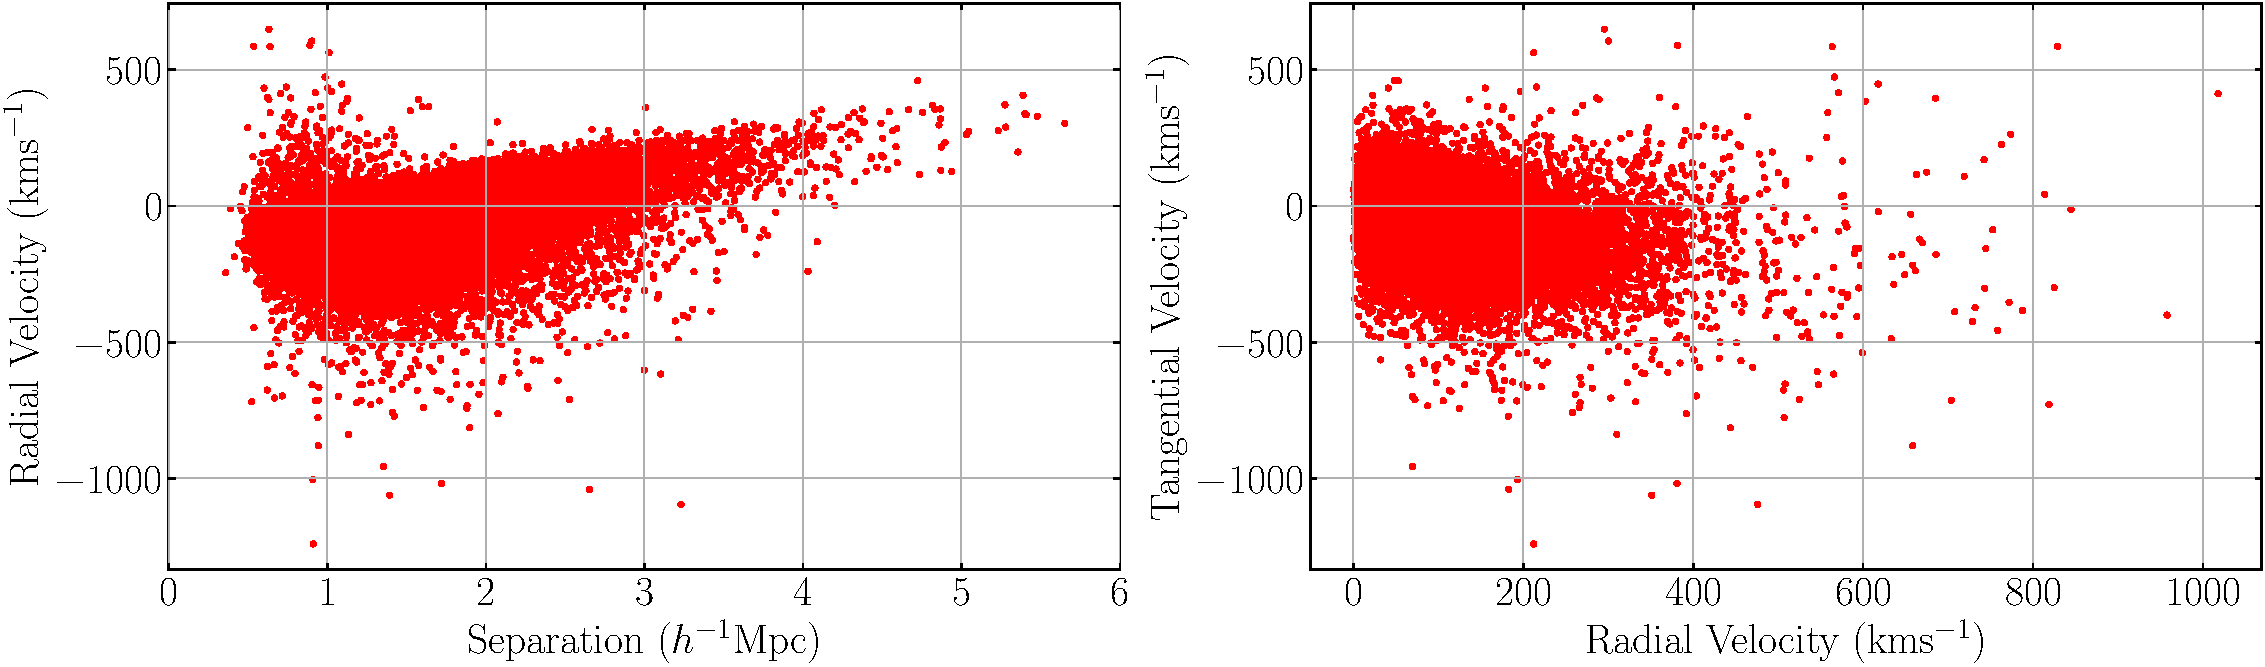
\includegraphics[width=1.0\textwidth]{both_06.pdf}
\end{center}
\caption{In left panel radial velocity distribution in term of halos separation. Right panel show 2D histograms for LG-like halo pairs.} 
\label{fig:distri_total}
\end{figure*}

From the IP sample we select the pairs with some similarity to the observed LG. The conditions we impose are the following: the maximum circular velocity should for both halos in the pair must be less than $250$ \kms, the relative radial velocity should be negative and the magnitude of the tangential velocity should be lower than the magnitude of the radial velocity. We refer to this sample simply as the pair sample. Only about $1\%$ of the halos in the initial sample are found in the pair sample. This is consistent with previous results that show that the fraction of LG pairs in a cosmological context.

Figure \ref{fig:distri_total} shows the relative peculiar velocities plotted from the halos separation in left panel. There is a marked tendency for close pairs to have a negative velocity. The right panel of the same figure shows the dispersion of halos in terms of their properties in radial and tangential relative velocity respectively. For this sample we have that a maximum for the most probable pairs is found in $v_{radial}=-52.83\pm 28.57$ \kms and $v_{tangential}=74.88\pm 36.89$ \kms. Distribution of radial and tangential velocities is in accord with larger distributions and reported results.

\section{Results}
In the figure \ref{fig:proba}, we plot a histogram for the velocity distribution for both isolated pairs and paired halos. Paired halos show slightly lower density than isolated pairs, particularly for peculiar velocities greater than 627 \kms. We can also observe that about 17 percent of the isolated halos and 16 percent of the matched halos have peculiar speeds greater than 627 \kms. This probability density is calculated for a model box with $H=67.9$ \kms \hMpc, $\lambda=0.693$, $\Omega_m=0.307$, $\sigma_8=0.831$, $w_0=-0.934$, and spectral index $n_s=0.97$. As we can see in the cumulative probability density, halos in isolated pairs tend to have lower peculiar velocities than the general sample of individual halos.

\begin{figure*}
\begin{center}
  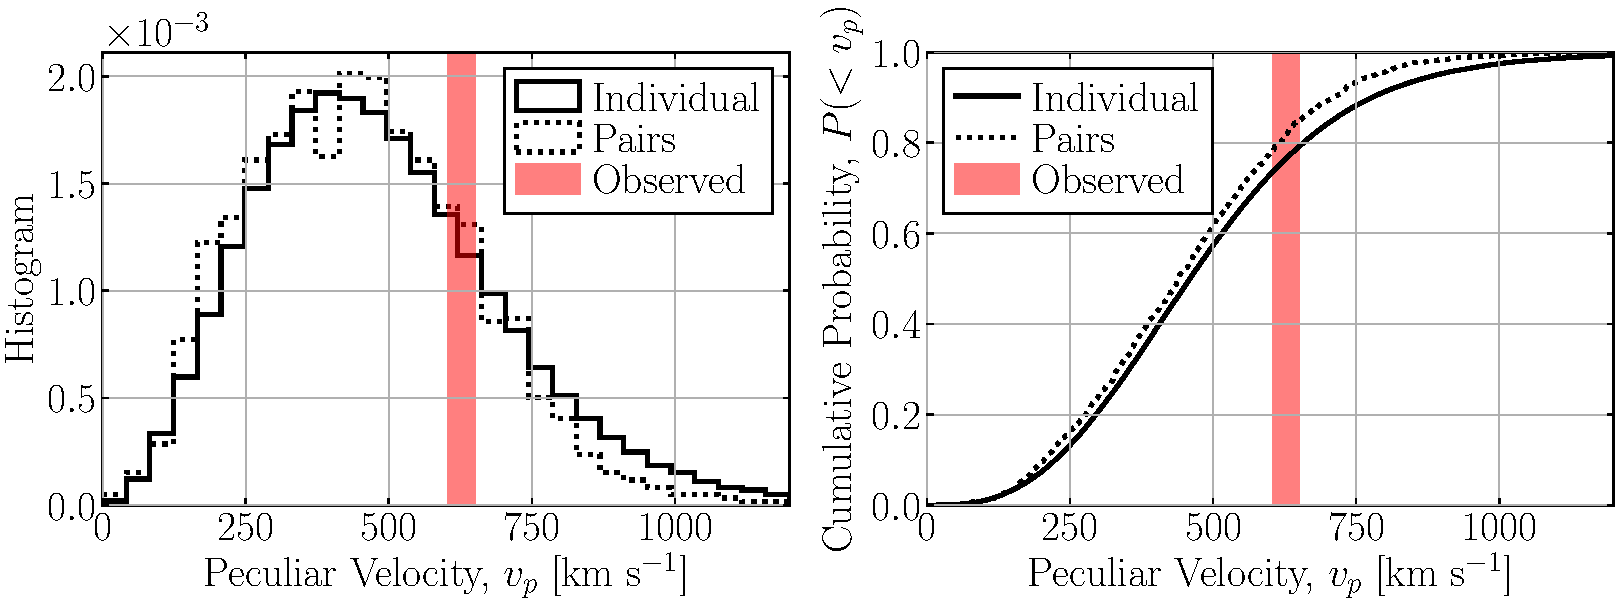
\includegraphics[width=0.9\textwidth]{cumulative_probability_18.pdf}
\end{center}
\caption{Distributions of peculiar velocities for MW type halos (individual, paired and observed). 
  Left panel shows the estimated probability density.
  The right panel shows the cumulative probability density. Paired halos have a slightly lower peculiar velocity than isolated halos. The observed peculiar velocity ($v_p=627\pm22$ km s$^{-1}$) shown as the vertical shaded stripe, is always located on the high velocity tail of simulations.
  Halos in isolated pairs tend to have lower peculiar velocities than the general sample of individual halos.}
\label{fig:proba}
\end{figure*} 

For a large sample of isolated dark matter halo pairs drawn from cosmological N-body simulations we can identify candidate systems whose kinematics match that of the Local Group galaxies. These simulations reproduce, by construction, the main kinematics of the MW–M31 pair. In this case (Figures \ref{fig:ratio_total} and \ref{fig:ratio_fast}), We can see that fast halos with speeds greater than $v_p=627\pm22$ km s$^{-1}$  have lower densities than the total halos found with properties similar to those of the LG. 0.07\%$\pm$0.01\% and 0.43\%$\pm$0.06\% are the densities of halos found with kinematics close to those of LG for fast and total halos respectively. From simulations we found that (over certain conditions) peculiar velocities from individual and paired halos have a dispersion of $445.76\pm 203.52$ \kms and $421.87\pm 185.68$, respectively. 

\begin{figure*}
\begin{center}
  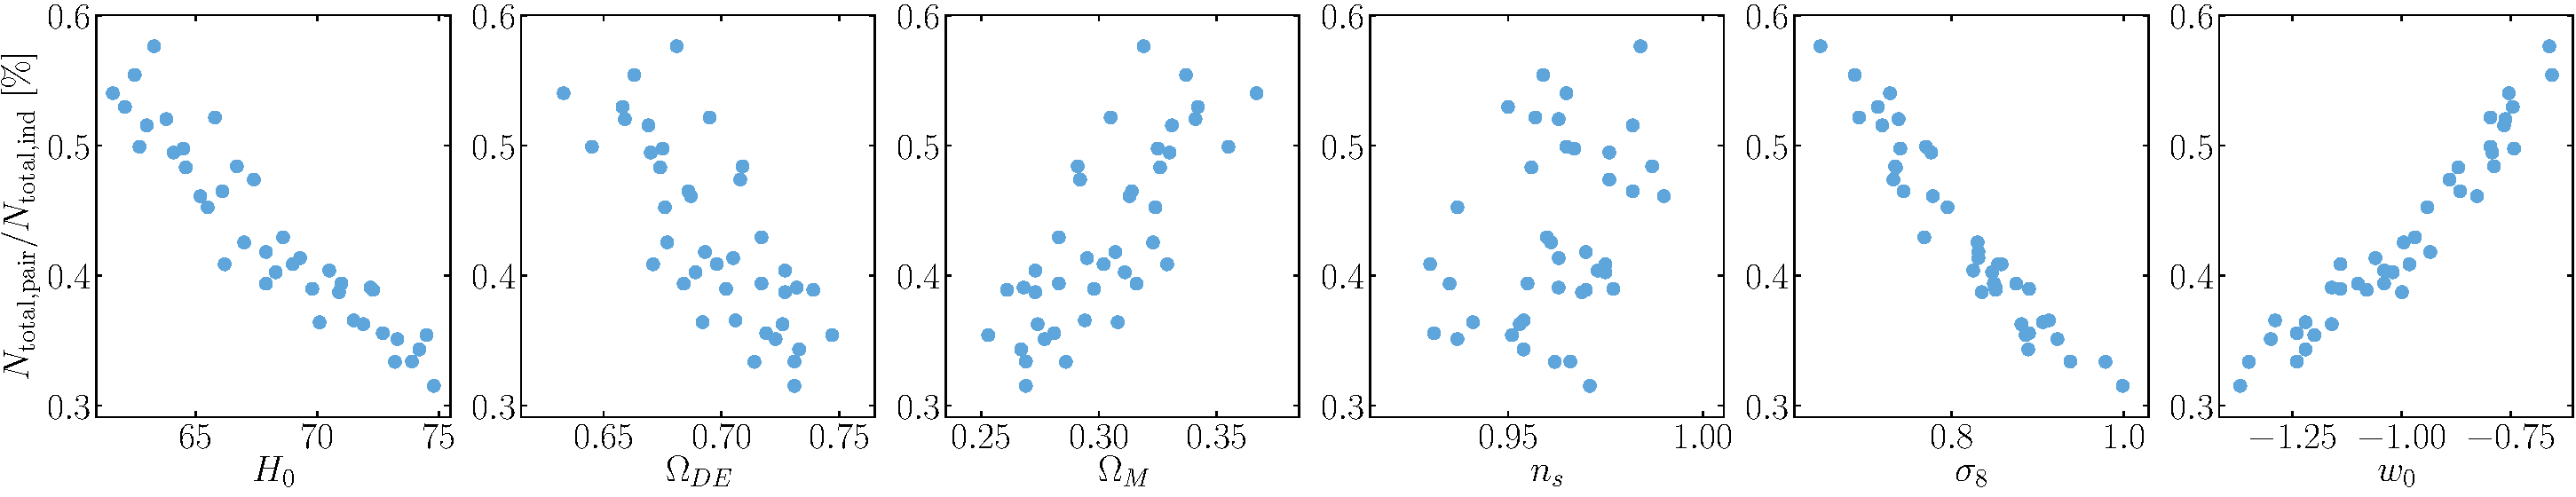
\includegraphics[width=1.0\textwidth]{ratio_pair_total_ind_total.pdf}
\end{center}
\caption{Ratio of the number of halos in pairs to the total number of isolated halos as a function of the cosmological parameters in the abacus simulations. Across simulations only $0.43 (\pm 0.06) \%$ of the halos can be found in pairs with kinematics and isolation similar to the MW-M31 pair.} 
\label{fig:ratio_total}
\end{figure*}

\begin{figure*}
\begin{center}
  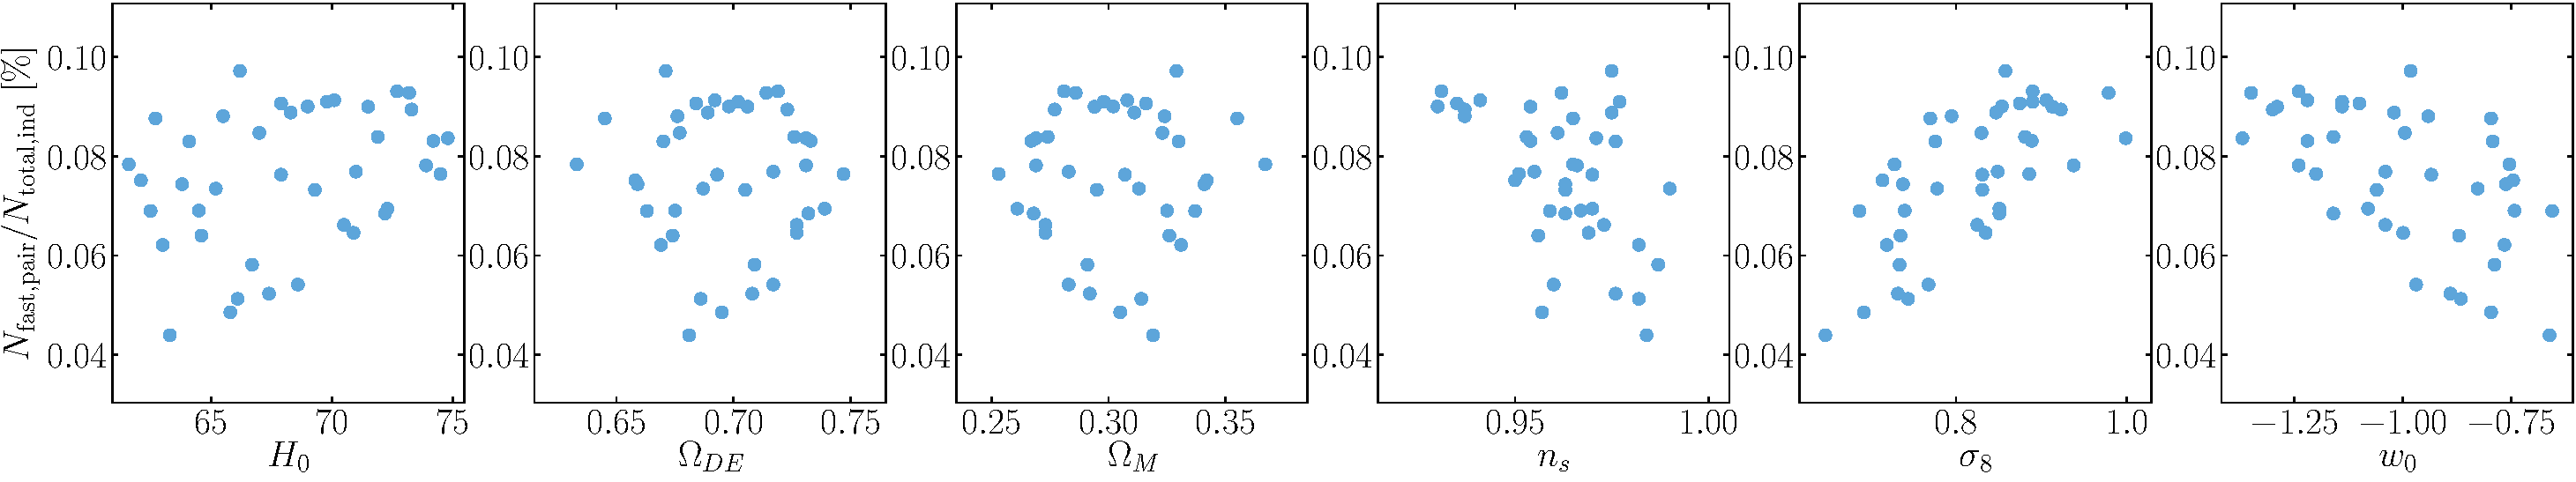
\includegraphics[width=1.0\textwidth]{ratio_pair_high_ind_total.pdf}
\end{center}
\caption{Ratio of the number of fast halos in pairs to the total number of isolated halos as a function of the cosmological parameters in the abacus simulations. Only $0.07 (\pm0.01) \%$ of the halos have similar kinematic conditions as the MW-M31 pairs.}
\label{fig:ratio_fast}
\end{figure*}

In order to measure the halos alignment in sample, we use $\hat v_p$ and $\hat r_{AB}$ (the peculiar velocity and the position of paired halos). Figure \ref{fig:alignment} displays the cosine of angle cumulative distribution between both vectors. For this study we found that 61\% and 72\% of Fast Pairs (defined as pairs with peculiar velocity greater of $v_p=627\pm22$ \kms) and All Pairs have values of cosine angles less than observed from CMB anisotropy dipole atributed to the Solar System motion respect to the CMB rest frame. This behavior is in agreement with earlier studies of the velocity anisotropy of subhalos, which is usually expressed by the anisotropy parameter $\beta=1-0.5(\sigma_{t}/\sigma_{r})^{2}$ (e.g., \cite{1987gady.book.....B}. Halos that possess peculiar peculiar relative speeds align with their closest partner. Fast halos differ in strength respect of all halos considered in simulation, the halo alignment it's less intense for fats halos.

\begin{figure*}
\begin{center}
  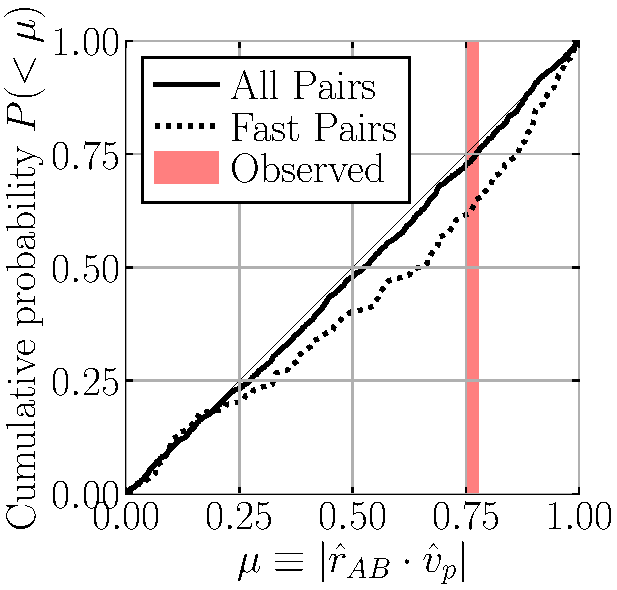
\includegraphics[width=0.4\textwidth]{cumulative_alignment_06.pdf}
\end{center}
\caption{Cumulative probability for the dot product between the unit vector joining the two halos in the pair and the peculiar velocity of the less massive halo.  Continous line: results for all pairs; dashed line: pairs where the less massive halo moves with a pecular velocity larger than $v_p=627\pm22$ km s$^{-1}$. The vertical stripe shows the values for the MW and M31. Halos with high peculiar velocities tend to be aligned in the direction towards its partner.}
\label{fig:alignment}
\end{figure*}

\section{Conclusions}
We have analyzed the kinematics exhibited by simulated halo candidates from N-body simulations that possess properties similar to pairs of galaxies encoded in the LG, such as MW-M31. We have used these similarities to guide selection, from a set of cosmological simulations. The Abacus project determines cosmologically representative volumes using stellar mass functions of galaxies and average galaxy sizes in good agreement with existing observations and cosmologies.
We also compared the population of simulated galaxies with those observed visually in MW-M31 systems.
Our main conclusions are summarized in the following:
\begin{itemize}
\item The kinematics of MW-M31 type pairs that find a similar in cosmological simulations and other members of the LG are consistent with the observations. We obtain that from a remarkable anisotropy, about 1/6 of the individual pairs and paired halos have peculiar velocities greater than those found in the observations ($627 \pm 22$ \kms), being slightly less dense the paired halos in the simulation sample. The velocities dispersion of the simulated halos are consistent with those found in MW-M31 type pairs.
\item We found a higher correlation in paired halos with respect to cosmological parameters, than those found in fast halos ($v_p> 627 \pm 22$ \kms) and also, fast halos exhibited a slightly higher density than individual halos.
\item Rapid halos also have a lower density with respect to the individual halos as a function of their alignment with respect to the resting CMB system.
\end{itemize}

\bibliographystyle{mnras}
\bibliography{references}



\end{document}
